\documentclass[border=4pt]{standalone}
\usepackage{amsmath,amssymb}
\usepackage{tikz}
\begin{document}
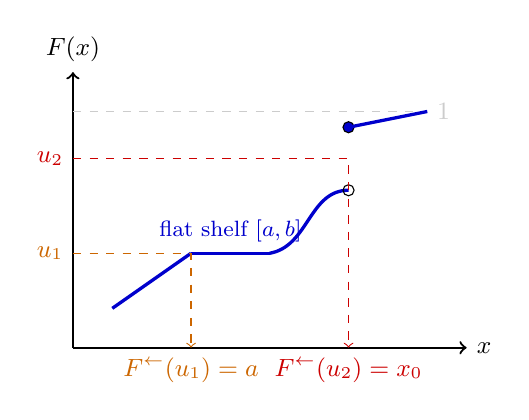
\begin{tikzpicture}[font=\small]
  \draw[->, thick] (0,0) -- (5.0,0) node[right] {$x$};
  \draw[->, thick] (0,0) -- (0,3.5) node[above] {$F(x)$};

  \draw[dashed, gray!40] (0, 3.0) -- (4.5, 3.0) node[right] {$1$};

  % CDF curve with shelf and jump
  \draw[very thick, blue!80!black] (0.5, 0.5) -- (1.5, 1.2);
  \draw[very thick, blue!80!black] (1.5, 1.2) -- (2.5, 1.2) node[midway, above, font=\footnotesize] {flat shelf $[a,b]$};
  \draw[very thick, blue!80!black] (2.5, 1.2) to[out=10, in=180] (3.5, 2.0);
  \draw (3.5, 2.0) circle (2pt);
  \draw[fill=blue!80!black] (3.5, 2.8) circle (2pt);
  \draw[very thick, blue!80!black] (3.5, 2.8) -- (4.5, 3.0);

  % Inverse mappings
  \draw[dashed, orange!80!black, ->] (0, 1.2) node[left] {$u_1$} -- (1.5, 1.2) -- (1.5, 0) node[below] {$F^\leftarrow(u_1)=a$};
  \draw[dashed, red!80!black, ->] (0, 2.4) node[left] {$u_2$} -- (3.5, 2.4) -- (3.5, 0) node[below] {$F^\leftarrow(u_2)=x_0$};
\end{tikzpicture}
\end{document}